\documentclass[11pt,a4paper]{article}
\usepackage[utf8]{inputenc}
\usepackage[T1]{fontenc}
\usepackage[spanish,es-noshorthands]{babel}
\usepackage{amsmath,amssymb,amsthm}
\usepackage{bm}
\usepackage{geometry}
\geometry{margin=2.5cm}
\usepackage{graphicx}
\graphicspath{{../figuras/}}
\usepackage{float}
\usepackage{xcolor}
\usepackage{hyperref}
\hypersetup{colorlinks=true,linkcolor=blue!50!black,citecolor=blue!50!black,urlcolor=blue!50!black}
\usepackage{enumitem}
\usepackage{booktabs}
\newtheorem{definition}{Definición}
\newtheorem{remark}{Observación}
\newcommand{\R}{\mathbb{R}}
\newcommand{\thetavec}{\bm{\theta}}
\newcommand{\transp}{^{\top}}
\newcommand{\promptIA}[1]{\begin{center}\fcolorbox{gray}{gray!8}{\parbox{0.9\linewidth}{\small\textbf{[FIGURA -- PROMPT IA]}\\[2pt]#1}}\end{center}}
\title{\textbf{B2 --- Poblaciones neuronales y el balance excitación/inhibición}\\[2pt]\large El nivel de descripción del modelo de Wilson--Cowan}
\author{Proyecto Wilson--Cowan --- Iniciación a la I+D ITBA}
\date{\today}
\begin{document}
\maketitle
\tableofcontents
\bigskip

\section{Modelos de tasa y de campo medio: qué promedian y qué pierden}

En B1 vimos la neurona individual: canales iónicos, potencial de membrana, spikes. Si quisiéramos describir un pedazo de corteza así, tendríamos que simular decenas de miles de neuronas, cada una con sus ecuaciones. Ni es tratable computacionalmente ni es lo que queremos: para preguntas sobre \emph{ritmos} cerebrales (oscilaciones theta, gamma) no nos importa qué hace la neurona número 4\,732, sino qué hace la \emph{población}.

\begin{definition}[Modelo de tasa, \emph{rate model}]
Un modelo de tasa reemplaza el tren de spikes de una neurona (o de un grupo de neuronas) por una única variable continua $r(t)\ge 0$: la \emph{tasa de disparo} (\emph{firing rate}), es decir, cuántos spikes por segundo emite la población en promedio alrededor del instante $t$.
\end{definition}

La idea de \textbf{campo medio} (\emph{mean-field}) es un paso más: en vez de seguir a cada neurona de una población, se supone que todas reciben aproximadamente la misma entrada promedio y se las resume en una sola variable de actividad. Se pasa de $N$ ecuaciones (una por neurona) a \emph{una} ecuación por población. Es exactamente la misma jugada que en física estadística: no seguís cada molécula de un gas, seguís presión y temperatura.

\paragraph{Qué se gana.} Tratabilidad y comprensión. Con dos o tres variables (una por población) tenemos un sistema de EDOs de baja dimensión (ver M2, EDOs y sistemas dinámicos), al que se le puede hacer retrato de fase, buscar equilibrios, estudiar bifurcaciones. Es \emph{este} nivel el que hace posible todo nuestro proyecto: identificar 10 parámetros por Neural ODE, diagnosticar con Fisher+SVD, cerrar un lazo de control. Nada de eso sería viable sobre un modelo spike-a-spike de $10^4$ neuronas.

\paragraph{Qué se pierde.} Al promediar, tiramos información:
\begin{itemize}[leftmargin=1.4em,itemsep=2pt]
  \item \textbf{Spikes individuales.} El modelo entrega una tasa suave; no hay potenciales de acción discretos. No podés preguntarle por el tiempo exacto de un spike.
  \item \textbf{Sincronía fina.} La aproximación de campo medio supone que las neuronas de una población están, en promedio, en un estado parecido. Correlaciones finas de \emph{spike-timing} entre neuronas (la estructura microscópica de la sincronía) quedan fuera.
  \item \textbf{Heterogeneidad.} Diferencias neurona-a-neurona (umbrales, conexiones) se lavan en el promedio.
\end{itemize}

\begin{remark}
Que ``se pierda'' la sincronía fina no significa que se pierdan las \emph{oscilaciones}. Wilson--Cowan captura ritmos poblacionales sostenidos (la tasa sube y baja periódicamente) sin representar el spike-timing de cada neurona. Es un modelo de la \emph{envolvente} de actividad, no de los spikes.
\end{remark}


\section{Dos poblaciones, E e I, y la conectividad recurrente}

Wilson y Cowan (1972) hicieron la elección mínima que todavía captura la física del asunto: \emph{dos} poblaciones acopladas.

\begin{itemize}[leftmargin=1.4em,itemsep=2pt]
  \item Una población \textbf{excitatoria} $E$: sus neuronas, al disparar, \emph{aumentan} la actividad de aquellas a las que proyectan (piensen en piramidales glutamatérgicas).
  \item Una población \textbf{inhibitoria} $I$: al disparar, \emph{reducen} la actividad de sus blancos (interneuronas GABAérgicas).
\end{itemize}

La clave es que el acople es \textbf{recurrente}: cada población se proyecta a la otra y a sí misma. Eso da cuatro caminos, y a cada uno le corresponde un \emph{peso} sináptico efectivo (cuán fuerte es esa conexión a nivel poblacional):

\begin{center}
\begin{tabular}{clc}
\toprule
Peso & Conexión & En el simulador \\
\midrule
$w_{EE}$ & $E \to E$ \; (autoexcitación) & 6.4 \\
$w_{IE}$ & $E \to I$ \; (E activa a I) & 6.0 \\
$w_{EI}$ & $I \to E$ \; (I frena a E) & 4.8 \\
$w_{II}$ & $I \to I$ \; (autoinhibición) & 1.2 \\
\bottomrule
\end{tabular}
\end{center}

\begin{remark}[Convención de subíndices]
Leemos $w_{XY}$ como ``peso del efecto que $Y$ ejerce sobre $X$'': $w_{EI}$ es cuánto pesa $I$ en la entrada de $E$. Ojo con esto al leer las ecuaciones: en la entrada de $E$ aparece $+w_{EE}E - w_{EI}I$ (la propia $E$ suma, la $I$ resta), y en la de $I$ aparece $+w_{IE}E - w_{II}I$. Los signos de resta ($w_{EI},w_{II}$) codifican que $I$ inhibe.
\end{remark}

Además de las conexiones internas, cada población recibe una \textbf{entrada externa}: $P(t)$ va a la población $E$ y $Q(t)$ va a la población $I$. En nuestro proyecto, $P$ y $Q$ son los estímulos de control (pensados para ser realizables con optogenética: señales $\ge 0$, tipo on/off). El esquema completo está en la Figura~\ref{fig:red}.

\begin{figure}[H]
\centering
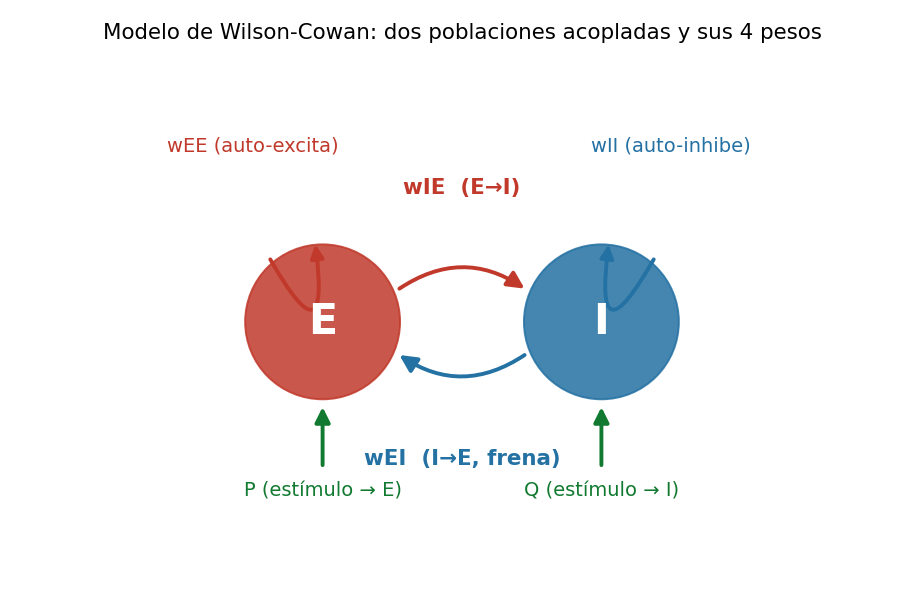
\includegraphics[width=0.75\linewidth]{fig_red_EI.png}
\caption{Esquema de la red de Wilson--Cowan: las dos poblaciones $E$ (excitatoria) e $I$ (inhibitoria), los cuatro pesos recurrentes $w_{EE},w_{IE},w_{EI},w_{II}$ y las entradas externas $P\to E$, $Q\to I$. (figura del proyecto)}
\label{fig:red}
\end{figure}

Con esta red, y usando la forma canónica del modelo que adoptamos en el proyecto (estado $\mathbf{x}=[I,E]$, salida observada $y=E-I$), las ecuaciones son:
\begin{align}
\dot I &= \tfrac{1}{\tau_i}\big(-I + S_i(w_{IE}E - w_{II}I + Q(t) - \theta_i) - k_i\big),\\[2pt]
\dot E &= \tfrac{1}{\tau_e}\big(-E + S_e(w_{EE}E - w_{EI}I + P(t) - \theta_e) - k_e\big).
\end{align}
El desarrollo completo de estas ecuaciones y de sus 10 parámetros es materia de B3 (modelo de Wilson--Cowan); acá nos quedamos con la lectura de red. Los términos $k_e,k_i$ son offsets que se \emph{restan} para que el reposo $E=I=0$ sea un equilibrio cuando no hay estímulo; se derivan, no se aprenden libres.


\section{La sigmoidea como función de activación poblacional}

Dentro de cada ecuación aparece una función $S(\cdot)$: la \textbf{función de activación} de la población. Es una sigmoidea (curva en S):
\begin{equation}
S_a(u)=\frac{1}{1+e^{-a\,(u)}},
\end{equation}
que toma la \emph{entrada total} $u$ que llega a la población (suma de pesos por actividades, más estímulo externo, menos umbral) y devuelve la \emph{fracción de la población que se activa}, entre 0 y 1.

\paragraph{Por qué una sigmoidea, y no una recta.} La forma en S no es un capricho matemático: refleja dos saturaciones reales de una población de neuronas.
\begin{itemize}[leftmargin=1.4em,itemsep=2pt]
  \item \textbf{Piso.} Si la entrada es muy baja, casi ninguna neurona supera su umbral: la actividad poblacional $\approx 0$. La curva se aplana abajo.
  \item \textbf{Techo.} Si la entrada es muy alta, ya casi todas las neuronas disparan: no se puede más. La curva satura arriba.
  \item \textbf{Zona sensible.} En el medio, un pequeño cambio de entrada mueve mucho la actividad: es la región de trabajo interesante, donde la población ``decide''.
\end{itemize}

La sigmoidea tiene dos parámetros con lectura biológica directa (Figura~\ref{fig:sig}):
\begin{itemize}[leftmargin=1.4em,itemsep=2pt]
  \item \textbf{Ganancia $a$ (pendiente).} Cuán empinada es la S en su zona sensible. Ganancia alta $\Rightarrow$ población casi de tipo interruptor (apagado/encendido); ganancia baja $\Rightarrow$ respuesta gradual, ``blanda''. En el simulador, $a_e=1.2$ y $a_i=1.0$.
  \item \textbf{Umbral $\theta$ (dónde enciende).} El valor de entrada al que la población llega a la mitad de su rango: desplaza la curva a izquierda/derecha. Umbral alto $\Rightarrow$ hace falta más entrada para encender. En el simulador, $\theta_e=2.8$ y $\theta_i=4.0$.
\end{itemize}

\begin{figure}[H]
\centering
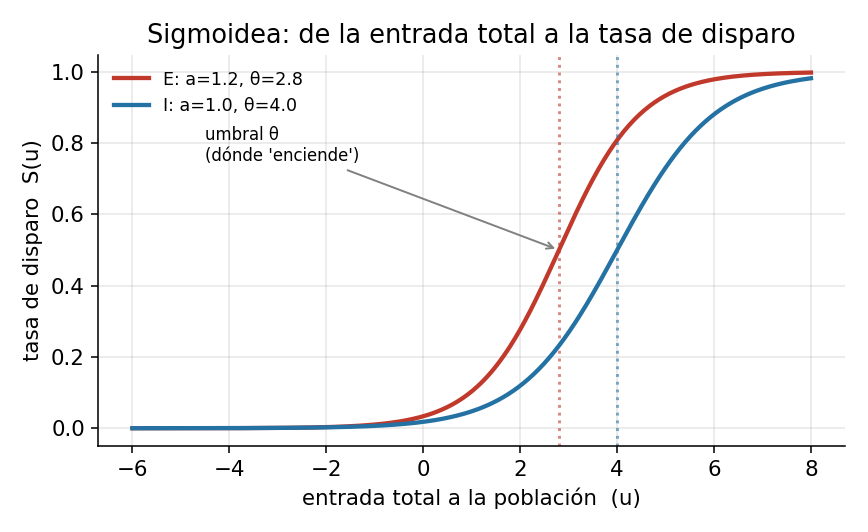
\includegraphics[width=0.75\linewidth]{fig_sigmoidea.png}
\caption{La función de activación poblacional $S(u)$ para $E$ e $I$: entrada total en el eje horizontal, fracción de población activa en el vertical. Se señalan el umbral $\theta$ (dónde la curva llega a la mitad) y el efecto de la ganancia $a$ (la pendiente). (figura del proyecto)}
\label{fig:sig}
\end{figure}

\begin{remark}[Por qué nos importa en el proyecto]
Cuatro de los diez parámetros que identificamos son de estas sigmoideas: $a_e,a_i,\theta_e,\theta_i$. Además, la sigmoidea es la \emph{no linealidad} del sistema: sin ella el modelo sería lineal y no podría oscilar de forma sostenida. Es la fuente de toda la dinámica rica, y también de que el problema de identificación sea no trivial.
\end{remark}


\section{El balance excitación/inhibición (E/I)}

Ya tenemos las piezas: dos poblaciones que se empujan (E) y se frenan (I) mutuamente, cada una con su constante de tiempo ($\tau_e=1.0$, $\tau_i=2.0$: la inhibición es \emph{más lenta}). El corazón del comportamiento de Wilson--Cowan es el \textbf{tira y afloja} entre E e I.

\paragraph{El mecanismo del oscilador.} Sigamos el bucle:
\begin{enumerate}[leftmargin=1.6em,itemsep=2pt]
  \item Un empujón sube $E$ (se autoexcita vía $w_{EE}$).
  \item Esa $E$ alta activa a $I$ (vía $w_{IE}$)\ldots pero $I$ es más lenta, llega con retraso.
  \item Cuando $I$ finalmente sube, frena a $E$ (vía $w_{EI}$): $E$ cae.
  \item Sin $E$ que la alimente, $I$ también decae\ldots y el ciclo puede recomenzar.
\end{enumerate}
Ese desfase entre ``E sube'' e ``I responde tarde'' es lo que produce, para pesos y entradas adecuados, un \textbf{ciclo límite}: una oscilación sostenida y autónoma (ver M2 para la noción de ciclo límite). Es el mismo principio de un depredador--presa: las presas crecen, luego los depredadores, que las diezman, luego los depredadores mueren de hambre, y vuelta a empezar.

\begin{remark}[Un detalle numérico del proyecto]
Con los pesos por defecto (Sección~2), el que el sistema oscile o no depende del estímulo. Con $P\approx 1.2$, $Q\approx 0.6$ el sistema entra en ciclo límite (oscila). Con $P=0.8$, $Q=0.6$ cae en un foco estable (se apaga hacia un equilibrio). Mismo cerebro, distinto régimen según la entrada: eso es lo que explota el control.
\end{remark}

\paragraph{Relevancia funcional.} El balance E/I no es solo el que enciende oscilaciones: es el que las mantiene \emph{en su punto}. Un E/I bien regulado permite ritmos estables (theta, gamma), respuestas graduadas y capacidad de conmutar entre estados. El régimen que nos interesa en el proyecto es \textbf{theta--gamma}: ráfagas rápidas (gamma) moduladas por una envolvente lenta (theta), un código propuesto para memoria de trabajo. Ese acoplamiento de dos escalas de tiempo nace, precisamente, de la interacción E/I con constantes de tiempo distintas.

\paragraph{Cuando el balance se rompe: patología.} Si la excitación domina sistemáticamente sobre la inhibición (E/I ``roto'' hacia arriba), el bucle de freno falla: $E$ crece sin que $I$ la contenga, y la actividad se descontrola en una descarga hipersincrónica. Ése es el correlato de la \textbf{epilepsia}: exceso de excitación / inhibición insuficiente. No es casual que uno de los usos de la optogenética que motiva nuestros estímulos (Krook-Magnuson et al., 2013) sea justamente frenar convulsiones ``a demanda'' reactivando inhibición. Entender y poder \emph{controlar} el balance E/I es, en el fondo, la motivación clínica del proyecto.


\section{Dónde vive Wilson--Cowan en la jerarquía de modelos}

Wilson--Cowan no es ``el'' modelo del cerebro: es \emph{un nivel de descripción}, elegido a propósito. Vale la pena ubicarlo en la escalera, de lo más microscópico a lo más macroscópico. En cada escalón se gana algo y se pierde algo (Cuadro~\ref{tab:jerarquia}).

\begin{enumerate}[leftmargin=1.6em,itemsep=3pt]
  \item \textbf{Hodgkin--Huxley (biofísico, spike a spike).} Ecuaciones para las corrientes iónicas (Na$^+$, K$^+$) que generan cada potencial de acción. \emph{Gana:} realismo biofísico, predice la forma del spike. \emph{Pierde:} tratabilidad: 4 variables no lineales \emph{por neurona}, imposible de escalar a poblaciones o de identificar de forma limpia.
  \item \textbf{Integrate-and-fire.} La neurona se reduce a acumular voltaje y disparar al cruzar un umbral, reseteando. \emph{Gana:} muchísima simplicidad, todavía spikes. \emph{Pierde:} el detalle de los canales; la forma del spike es un evento impuesto, no emergente.
  \item \textbf{Modelos de tasa (\emph{rate models}).} Se abandona el spike; la variable es la tasa de disparo (Sección~1). \emph{Gana:} variable continua, apta para EDOs y análisis dinámico. \emph{Pierde:} el spike-timing individual.
  \item \textbf{Neural mass --- \emph{Wilson--Cowan}.} Un modelo de tasa donde cada \emph{población} (E, I) es una masa con su variable de actividad, acopladas por los cuatro pesos. \emph{Gana:} dos o tres variables describen un pedazo de corteza; oscilaciones poblacionales, retrato de fase, identificación de parámetros. \emph{Pierde:} toda la estructura interna de la población y el espacio (todo pasa ``en un punto''). \textbf{Éste es nuestro nivel.}
  \item \textbf{Neural field --- Wilson--Cowan espacial.} Se le devuelve el \emph{espacio}: $E$ e $I$ pasan a ser campos $E(x,t),I(x,t)$ sobre la corteza, con núcleos de conectividad que dependen de la distancia. \emph{Gana:} ondas viajeras, patrones espaciales, actividad que se propaga. \emph{Pierde:} simplicidad; es una ecuación integro-diferencial, mucho más costosa. En nuestro proyecto trabajamos con la versión \emph{sin} espacio (neural mass), suficiente para theta--gamma y control.
\end{enumerate}

\begin{table}[H]
\centering
\small
\begin{tabular}{@{}p{3.2cm}p{4.2cm}p{4.6cm}@{}}
\toprule
\textbf{Nivel} & \textbf{Gana} & \textbf{Pierde} \\
\midrule
Hodgkin--Huxley & Realismo biofísico, forma del spike & Tratabilidad ($\sim$4 vars/neurona) \\
Integrate-and-fire & Simplicidad, aún hay spikes & Detalle de canales iónicos \\
Rate model & Variable continua, apta para EDOs & Spike-timing individual \\
\textbf{Neural mass (WC)} & \textbf{Pocas variables por población; oscilaciones, análisis, identificación} & \textbf{Estructura interna; espacio} \\
Neural field (WC espacial) & Ondas y patrones espaciales & Simplicidad y costo \\
\bottomrule
\end{tabular}
\caption{La jerarquía de modelos neuronales. Wilson--Cowan (neural mass) es el punto dulce para nuestro proyecto: suficientemente rico para oscilar, suficientemente simple para identificar y controlar.}
\label{tab:jerarquia}
\end{table}

\promptIA{Diagrama horizontal tipo ``escalera'' o flujo de izquierda (microscópico) a derecha (macroscópico) con cinco cajas conectadas por flechas: (1) ``Hodgkin--Huxley'' con un icono de un spike biofísico y canales iónicos; (2) ``Integrate-and-fire'' con un icono de voltaje que sube y se resetea; (3) ``Modelos de tasa'' con una curva de firing rate suave; (4) ``Neural mass: Wilson--Cowan'' resaltada en color (es el nivel del proyecto), con dos círculos E e I acoplados; (5) ``Neural field'' con una lámina cortical y una onda espacial. Debajo de la escalera, dos flechas largas opuestas: una etiquetada ``$\leftarrow$ más detalle biofísico, menos tratable'' y otra ``más tratable y abstracto $\rightarrow$''. Estilo científico limpio, fondo claro, etiquetas en español. Resaltar el escalón (4) como el foco.}

\begin{remark}[La moraleja]
Elegir un modelo es elegir qué preguntas querés poder contestar. Wilson--Cowan es el nivel donde ``balance E/I'', ``oscilación theta--gamma'' e ``identificar 10 parámetros para controlar'' son todas preguntas bien planteadas. Bajar a Hodgkin--Huxley las volvería intratables; subir a neural field agregaría espacio que no necesitamos.
\end{remark}


\begin{thebibliography}{9}
\bibitem{wc1972} H. R. Wilson y J. D. Cowan, ``Excitatory and inhibitory interactions in localized populations of model neurons'', \emph{Biophysical Journal} 12(1):1--24, 1972.
\bibitem{dayan} P. Dayan y L. F. Abbott, \emph{Theoretical Neuroscience: Computational and Mathematical Modeling of Neural Systems}, MIT Press, 2001.
\bibitem{deco2008} G. Deco, V. K. Jirsa, P. A. Robinson, M. Breakspear y K. Friston, ``The dynamic brain: from spiking neurons to neural masses and cortical fields'', \emph{PLoS Computational Biology} 4(8):e1000092, 2008.
\bibitem{gerstner} W. Gerstner, W. M. Kistler, R. Naud y L. Paninski, \emph{Neuronal Dynamics: From Single Neurons to Networks and Models of Cognition}, Cambridge University Press, 2014.
\bibitem{km2013} E. Krook-Magnuson, C. Armstrong, M. Oijala e I. Soltesz, ``On-demand optogenetic control of spontaneous seizures in temporal lobe epilepsy'', \emph{Nature Communications} 4:1376, 2013.
\end{thebibliography}

\end{document}
